\documentclass[aspectratio=169, 11pt]{beamer}

% ============================================
% THEME AND APPEARANCE
% ============================================

\usetheme{metropolis}
\usecolortheme{default}

% Custom colors
\definecolor{darkblue}{RGB}{0, 51, 102}
\definecolor{lightgray}{RGB}{245, 245, 245}
\definecolor{accentred}{RGB}{180, 30, 30}

\setbeamercolor{frametitle}{bg=darkblue, fg=white}
\setbeamercolor{title}{fg=darkblue}
\setbeamercolor{structure}{fg=darkblue}
\setbeamercolor{section in toc}{fg=darkblue}

% Remove navigation symbols
\setbeamertemplate{navigation symbols}{}

% Frame numbers
\setbeamertemplate{footline}[frame number]

% ============================================
% PACKAGES
% ============================================

\usepackage{graphicx}
\usepackage{booktabs}
\usepackage{amsmath,amssymb}
\usepackage{tikz}
\usetikzlibrary{arrows.meta, positioning}

% ============================================
% TITLE PAGE
% ============================================

\title{Necessity Entrepreneurs}
\subtitle{Occupational Choice, Misallocation, and Unemployment Insurance}
\author{David Chivers\inst{1} \and Zhigang Feng\inst{2} \and Elisa Keller\inst{3} \and Bo Li\inst{4}}
\institute{
    \inst{1} University of Durham \and
    \inst{2} University of Nebraska, Omaha \and
    \inst{3} University of Exeter \and
    \inst{4} Peking University
}
\date{2025}

\begin{document}

% ============================================
% SLIDE 1: TITLE
% ============================================

\begin{frame}[plain]
    \titlepage
\end{frame}

% ============================================
% SLIDE 2: AGENDA
% ============================================

\begin{frame}{Roadmap}
    \tableofcontents
\end{frame}

% ============================================
% SECTION 1: MOTIVATION
% ============================================

\section{Motivation}

% ============================================
% SLIDE 3: MOTIVATION
% ============================================

\begin{frame}{Motivation: Why This Matters}
    \begin{itemize}
        \item<1-> \textbf{Big picture:} Entrepreneurship drives innovation and growth
        \item<2-> \textbf{But:} Many entrepreneurs start businesses out of \textit{necessity}---not opportunity
        \item<3-> \textbf{Puzzle:} Negative correlation between entrepreneurship rates and development
        \item<4-> \textbf{Stakes:} Necessity entrepreneurship may signal \textcolor{accentred}{misallocation of talent}
    \end{itemize}

    \vspace{1em}

    \only<5>{
    \begin{block}{Key Distinction}
        \textbf{Opportunity entrepreneurs} choose entrepreneurship regardless of employment status \\
        \textbf{Necessity entrepreneurs} would \textit{not} start a business if they had a job
    \end{block}
    }
\end{frame}

% ============================================
% SLIDE 4: THIS PAPER
% ============================================

\begin{frame}{This Paper}
    \begin{center}
        \Large
        \textbf{Research Question:} \\[0.8em]
        How does unemployment risk shape \\
        the composition of entrepreneurship? \\[1.5em]
    \end{center}

    \textbf{What we do:}
    \begin{itemize}
        \item Build a span-of-control model with search frictions
        \item Endogenous occupational choice $\rightarrow$ two types of entrepreneurs emerge
    \end{itemize}

    \vspace{0.5em}

    \textbf{Preview of findings:}
    \begin{itemize}
        \item Unemployment insurance reduces necessity entrepreneurship
        \item Consumption floors have limited effect when UI is present
        \item Removing unemployment risk raises entrepreneurship across the board
    \end{itemize}
\end{frame}

% ============================================
% SECTION 2: MODEL
% ============================================

\section{Model}

% ============================================
% SLIDE 5: ECONOMIC ENVIRONMENT
% ============================================

\begin{frame}{Economic Environment}
    \textbf{Agents} differ in human capital $h$ (education: $P$, $S$, or $T$)

    \vspace{0.5em}

    $h$ determines:
    \begin{itemize}
        \item Managerial ability $x$ \quad (Pareto distributed)
        \item Labour productivity $z$
        \item Job separation rate $\rho$
    \end{itemize}

    \vspace{0.8em}

    \textbf{Production} \quad (Lucas span-of-control):
    \[
        y = x k^{\alpha}(zn)^{\gamma} \qquad \alpha, \gamma > 0
    \]

    \vspace{0.5em}

    \textbf{Labour market:} Search and matching frictions
    \begin{itemize}
        \item Employed workers face separation probability $\rho$
        \item Unemployed workers match with probability $p(\theta)$
        \item Government provides unemployment benefit $b$, financed by lump-sum tax $\tau$
    \end{itemize}
\end{frame}

% ============================================
% SLIDE 6: TIMING AND OCCUPATIONAL CHOICE
% ============================================

\begin{frame}{Timing and Occupational Choice}
    \begin{center}
    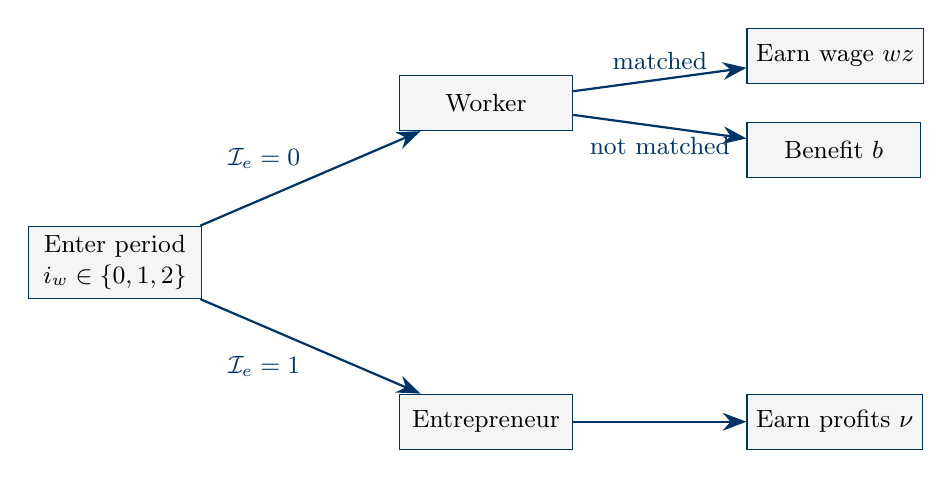
\begin{tikzpicture}[
        node distance=1.8cm and 2.5cm,
        every node/.style={font=\small},
        box/.style={rectangle, draw=darkblue, fill=lightgray, minimum width=2.2cm, minimum height=0.7cm, align=center},
        arrow/.style={-{Stealth[length=3mm]}, thick, darkblue}
    ]
        % Nodes
        \node[box] (start) {Enter period\\$i_w \in \{0,1,2\}$};
        \node[box, above right=1.2cm and 2.5cm of start] (worker) {Worker};
        \node[box, below right=1.2cm and 2.5cm of start] (entrep) {Entrepreneur};
        \node[box, right=2.2cm of worker, yshift=0.6cm] (matched) {Earn wage $wz$};
        \node[box, right=2.2cm of worker, yshift=-0.6cm] (unmatched) {Benefit $b$};
        \node[box, right=2.2cm of entrep] (profit) {Earn profits $\nu$};

        % Arrows
        \draw[arrow] (start) -- node[above left] {$\mathcal{I}_e=0$} (worker);
        \draw[arrow] (start) -- node[below left] {$\mathcal{I}_e=1$} (entrep);
        \draw[arrow] (worker) -- node[above] {matched} (matched);
        \draw[arrow] (worker) -- node[below] {not matched} (unmatched);
        \draw[arrow] (entrep) -- (profit);
    \end{tikzpicture}
    \end{center}

    \vspace{0.3em}

    \textbf{Key insight:} Employment status $i_w$ affects the \textit{outside option}, so it affects the entrepreneurship threshold $\hat{h}$
\end{frame}

% ============================================
% SLIDE 7: KEY MECHANISM
% ============================================

\begin{frame}{Key Mechanism: Two Types of Entrepreneurs}
    Let $\hat{h}$ be the critical human capital threshold for entrepreneurship.

    \vspace{0.5em}

    \textbf{Threshold depends on employment status:}
    \[
        \hat{h}_{i_w \neq 1} < \hat{h}_{i_w = 1}
    \]
    Unmatched workers have a \textit{lower} threshold $\rightarrow$ easier to push into entrepreneurship

    \vspace{1em}

    \begin{columns}[T]
        \begin{column}{0.48\textwidth}
            \textbf{\textcolor{darkblue}{Necessity Entrepreneurs}}
            \[
                \hat{h}_{i_w \neq 1} < h < \hat{h}_{i_w = 1}
            \]
            Would \textit{not} be entrepreneurs if employed
        \end{column}
        \begin{column}{0.48\textwidth}
            \textbf{\textcolor{darkblue}{Opportunity Entrepreneurs}}
            \[
                h \geq \hat{h}_{i_w = 1} \geq \hat{h}_{i_w \neq 1}
            \]
            Choose entrepreneurship \textit{regardless}
        \end{column}
    \end{columns}

    \vspace{0.8em}

    $\rightarrow$ Six critical thresholds total (2 per education level: $P$, $S$, $T$)
\end{frame}

% ============================================
% SECTION 3: QUANTITATIVE ANALYSIS
% ============================================

\section{Quantitative Analysis}

% ============================================
% SLIDE 8: CALIBRATION
% ============================================

\begin{frame}{Calibration}
    \begin{table}
        \centering
        \small
        \begin{tabular}{llll}
            \toprule
            Parameter & Value & Description & Source \\
            \midrule
            $\beta$ & 0.94 & Discount factor & \\
            $\sigma$ & 2.0 & Risk aversion & $u(c)=\frac{c^{1-\sigma}}{1-\sigma}$ \\
            $\alpha$ & 0.3207 & Capital share & \\
            $\gamma$ & 0.4693 & Labour share & Frac.\ of entrepreneurs \\
            $\bar{m}$ & 0.8 & Matching efficiency & Lubik (2013) \\
            $\mu$ & $[0.5, 0.7]$ & Matching elasticity & Petrongolo \& Pissarides \\
            $b$ & $0.40 \cdot w$ & UI benefits & Shimmer et al.\ (2005) \\
            $\rho$ & by $h$ & Separation rate & Cairo \& Cajner (2016) \\
            $z$ & by $h$ & Wage premium & Goldin \& Katz (2009) \\
            \bottomrule
        \end{tabular}
    \end{table}

    \vspace{0.3em}
    Three education levels ($P$, $S$, $T$) with population shares from Barro \& Lee (2013)
\end{frame}

% ============================================
% SLIDE 9: BASELINE RESULTS
% ============================================

\begin{frame}{Baseline Results: No Unemployment Counterfactual}
    \begin{table}
        \centering
        \small
        \begin{tabular}{lcc}
            \toprule
            & Baseline & No Unemployment \\
            \midrule
            Entrepreneur rate (avg) & 0.145 & 0.197 \\
            \quad Low education & 0.143 & 0.207 \\
            \quad Mid education & 0.137 & 0.184 \\
            \quad High education & 0.161 & 0.216 \\
            \midrule
            Firm size (avg) & 21.9 & 24.1 \\
            \quad Low education & 9.7 & 9.9 \\
            \quad Mid education & 18.0 & 19.8 \\
            \quad High education & 33.4 & 37.2 \\
            \midrule
            Unemp-Ent rate & 0.00204 & 0 \\
            \bottomrule
        \end{tabular}
    \end{table}

    \textbf{Takeaway:} Removing unemployment risk \textit{increases} entrepreneurship---all entrants are opportunity-driven, with larger firms
\end{frame}

% ============================================
% SLIDE 10: UI POLICY RESULTS
% ============================================

\begin{frame}{Policy Experiment: Unemployment Insurance}
    \begin{table}
        \centering
        \small
        \begin{tabular}{lccc}
            \toprule
            & Baseline & UI$=0.3$ & UI$=0.6$ \\
            & (UI$=0.4$) & & \\
            \midrule
            Entrepreneur rate (avg) & 0.145 & 0.145 & 0.144 \\
            \quad Low education & 0.143 & 0.141 & 0.135 \\
            \quad Mid education & 0.137 & 0.136 & 0.141 \\
            \quad High education & 0.161 & 0.164 & 0.154 \\
            \midrule
            Firm size (avg) & 21.9 & 21.6 & 21.2 \\
            Unemp-Ent rate & 0.00204 & 0.00197 & 0.00084 \\
            \bottomrule
        \end{tabular}
    \end{table}

    \vspace{0.5em}

    \textbf{Takeaway:} Higher UI benefits $\rightarrow$
    \begin{itemize}
        \item Necessity entrepreneurship falls (better outside option for unemployed)
        \item Average firm size declines modestly
        \item Low-education workers most responsive to UI changes
    \end{itemize}
\end{frame}

% ============================================
% SLIDE 11: CONSUMPTION FLOOR AND CREDIT
% ============================================

\begin{frame}{Further Experiments: Consumption Floor \& Credit Frictions}
    \textbf{Consumption floor} ($\underline{c}$): lump-sum transfer or utility penalty when income falls below threshold

    \vspace{0.5em}

    \begin{itemize}
        \item With UI present: consumption floor has \textbf{limited additional effect}
        \item Without unemployment: consumption floor barely moves entrepreneurship rates
    \end{itemize}

    \vspace{1em}

    \textbf{Credit friction wedge} ($\Delta$): borrowing cost premium for entrepreneurs

    \vspace{0.5em}

    \begin{itemize}
        \item Tighter credit $\rightarrow$ fewer entrepreneurs, smaller firms
        \item Interacts with asset holdings and occupational choice
    \end{itemize}

    \vspace{1em}

    $\rightarrow$ \textbf{UI design matters more} than consumption floors for reducing necessity entrepreneurship
\end{frame}

% ============================================
% SECTION 4: CONCLUSION
% ============================================

\section{Conclusion}

% ============================================
% SLIDE 12: TAKEAWAYS
% ============================================

\begin{frame}{Takeaways}
    \begin{enumerate}
        \item \textbf{Necessity entrepreneurs emerge endogenously} from the interaction of unemployment risk and occupational choice
        \item \textbf{Unemployment insurance reduces necessity entrepreneurship} by improving the outside option for jobless workers
        \item \textbf{Policy implication:} Well-designed UI can reduce misallocation of talent without substantially lowering overall entrepreneurship
    \end{enumerate}

    \vspace{2em}

    \begin{center}
        \Large Thank you! \\[0.5em]
        \normalsize david.chivers@durham.ac.uk
    \end{center}
\end{frame}

% ============================================
% APPENDIX
% ============================================

\appendix

\begin{frame}[noframenumbering]{Appendix: Household's Problem}
    \small
    \[
        \mathbf{V}(a,h,i_w) = \max_{\{a',c,p(\theta),\mathcal{I}_e\}}
        \begin{cases}
            \iota_{i_w=0}\left[(1-\mathcal{I}_e)\mathbb{E}_{p(\theta)}(\cdot) + \mathcal{I}_e(V_e + \beta\mathbb{E}\mathbf{V}(\cdot))\right] \\
            \iota_{i_w=1}\left[(1-\mathcal{I}_e)\mathbb{E}_{\rho}(\cdot) + \mathcal{I}_e(V_e + \beta\mathbb{E}\mathbf{V}(\cdot))\right] \\
            \iota_{i_w=2}\left[(1-\mathcal{I}_e)\mathbb{E}_{p(\theta)}(\cdot) + \mathcal{I}_e(V_e + \beta\mathbb{E}\mathbf{V}(\cdot))\right]
        \end{cases}
    \]

    subject to:
    \[
        c + a' \leq (1 + r - \delta)a + inc
    \]

    where $inc$ depends on occupation and employment status.
\end{frame}

\begin{frame}[noframenumbering]{Appendix: Firm's Problem}
    \small
    \textbf{Firm's profit maximization:}
    \[
        \max_{n,k} \; X k^{\alpha} n^{\gamma} - (1+\tau\psi)wzn - rk - \kappa \frac{\rho z n}{q(\theta)}
    \]

    \textbf{Optimal labor demand:}
    \[
        n^*(k,x,\tilde{w}) = \left[\frac{\gamma x k}{w(1+\psi\tau) + \frac{\rho\kappa}{q(\theta)}}\right]^{\frac{1}{1-\gamma}}
    \]

    \textbf{Matching function:}
    \[
        p(\theta) = \bar{m}\left(\frac{v}{u}\right)^{1-\mu}, \qquad q(\theta) = \bar{m}\left(\frac{v}{u}\right)^{-\mu}
    \]
\end{frame}

\end{document}
